\documentclass[../_main/handlingar.tex]{subfiles}


\begin{document}
\proposition{Inköp av cykelvagn}


Sektionen sköter idag stor del av sina transporter med kårens bil, Rulle, men då detta är förenat med en kostnad och för kortare transporter onödiga utsläpp så vore det bra med ett alternativ. Idag handlar källarmästeriet med cykel vilket fungerar men är otympligt och kräver att vi är tre personer som handlar tillsammans. Därför skulle det vara väldigt praktiskt med en cykelvagn att lasta med det vi behöver. Vagnen skulle också kunna användas av andra utskott till exempel för att transportera vatten och Soundboksen under nollningen. Den skulle kunna prydas med E-sektionens logga och därför ge bra uppmärksamhet som en hållbar och medveten sektion. 

Den föreslagna vagnen är av märket Christiania bikes och av god kvalitet vilket kan komma sektionen till nytta under lång tid framöver. Vagnen kan både dras för hand och kopplas till vilken cykel som helst. Vagnen kompletteras med ett regnskydd för användning i alla väder.\\ 
 
    \begin{center}
     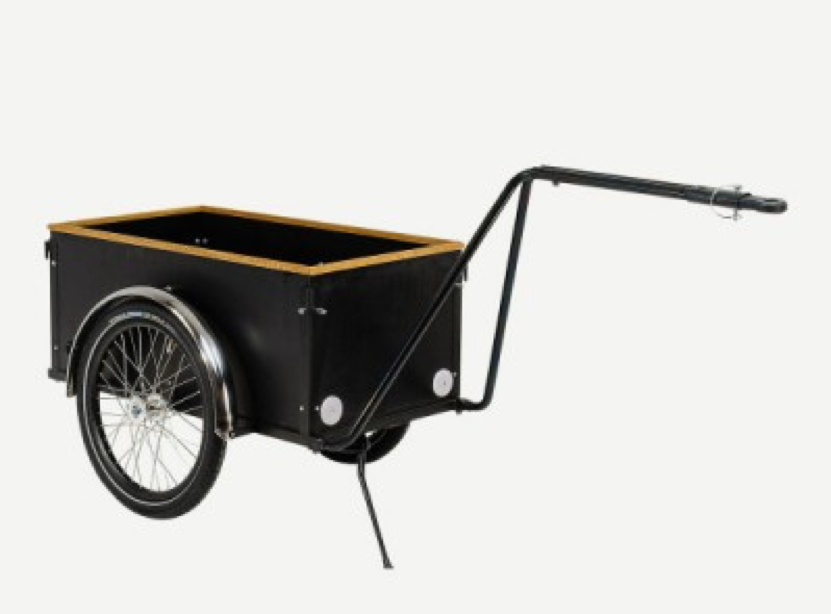
\includegraphics[scale=1]{../_res/vagn.png}
    \end{center}

\newpage

   \begin{tabular}{| l | l |}
    \hline
    Budget &  \\
     \hline
    \href{http://westlingscyklar.se/category/modeller/}{\textit{Cykelvagn extra bred (länk)}}  & \SI{5400}{kr}  \\
    \hline
    Frakt & \SI{995}{kr}\\
    \hline
    \href{http://westlingscyklar.se/category/talt/}{\textit{Regnskydd (länk)}}  & \SI{255}{kr}  \\
    \hline
    \href{https://www.kjell.com/se/sortiment/hem-kontor-fritid/cykeltillbehor/cykellas/abus-cykellas-med-kombinationskod-p21014 }{\textit{Lås (länk)}}  & \SI{209,90}{kr} kr  \\
    \hline
    Summa & \SI{6810}{kr} \\
    \hline
\end{tabular}

Styrelsen yrkar

\begin{attsatser}
    \att köpa in en cykelvagn av märket Christiania bikes med tillhörande regnskydd,
    \att budget sätts till \SI{7500}{kr}, 
    \att inköpet belastar utrustningsfonden, samt
    \att beslutet läggs på beslutsuppföljningen till Höstterminsmötet 2019 med undertecknad som ansvarig.
  
\end{attsatser}

\begin{signatures}{1}
    \ist
    \signature{\krog}{Krögare}
    
\end{signatures}

\end{document}
